\newpage
\mysection{ AVL Trees}

Copied From TutorialsPoint \href{https://www.tutorialspoint.com/data_structures_algorithms/avl_tree_algorithm.htm}{AvlTrees} \supcite{DataStru95:online}\\

What if the input to binary search tree comes in a sorted (ascending or descending) manner? It will then look like this:

\begin{center}
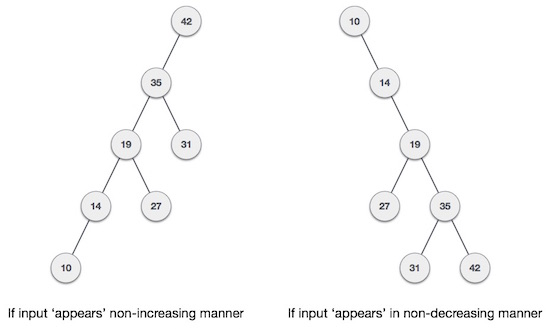
\includegraphics[scale=.60]{images/unbalanced_bst.jpg}
\end{center}

It is observed that BST's worst-case performance is closest to linear search algorithms, that is Ο(n). In real-time data, we cannot predict data pattern and their frequencies. So, a need arises to balance out the existing BST.\\

Named after their inventor \textbf{Adelson}, \textbf{Velski} \& \textbf{Landis}, \textbf{AVL trees} are height balancing binary search tree. AVL tree checks the height of the left and the right sub-trees and assures that the difference is not more than 1. This difference is called the \ccb{Balance Factor}.\\

Here we see that the first tree is balanced and the next two trees are not balanced −

\begin{center}
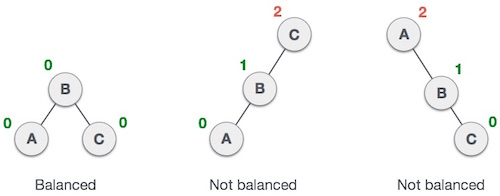
\includegraphics[scale=.60]{images/unbalanced_avl_trees.jpg}
\end{center}

In the second tree, the left subtree of \textbf{C} has height 2 and the right subtree has height 0, so the difference is 2. In the third tree, the right subtree of \textbf{A} has height 2 and the left is missing, so it is 0, and the difference is 2 again. AVL tree permits difference (balance factor) to be only 1.

\begin{verbatim}
BalanceFactor = height(left-sutree) − height(right-sutree)
\end{verbatim}

If the difference in the height of left and right sub-trees is more than \ccb{1}, the tree is balanced using some rotation techniques.

\newpage
\hypertarget{avl-rotations}{%
\mysubsection{AVL Rotations}\label{avl-rotations}}

To balance itself, an AVL tree may perform the following four kinds of rotations −

\begin{itemize}
\tightlist
\item
  Left rotation
\item
  Right rotation
\item
  Left-Right rotation
\item
  Right-Left rotation
\end{itemize}

The first two rotations are single rotations and the next two rotations are double rotations. To have an unbalanced tree, we at least need a tree of height 2. With this simple tree, let's understand them one by one.

\hypertarget{left-rotation}{%
\mysubsubsection{Left Rotation}\label{left-rotation}}

If a tree becomes unbalanced, when a node is inserted into the right subtree of the right subtree, then we perform a single left rotation −

\begin{center}
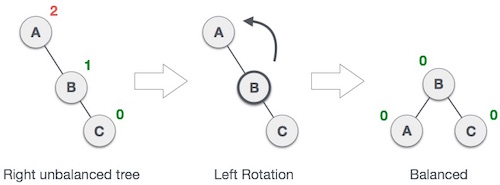
\includegraphics[scale=.60]{images/avl_left_rotation.jpg}
\end{center}

In our example, node \textbf{A} has become unbalanced as a node is inserted in the right subtree of A's right subtree. We perform the left rotation by making \textbf{A} the left-subtree of B.

\hypertarget{right-rotation}{%
\mysubsubsection{Right Rotation}\label{right-rotation}}

AVL tree may become unbalanced, if a node is inserted in the left subtree of the left subtree. The tree then needs a right rotation.

\begin{center}
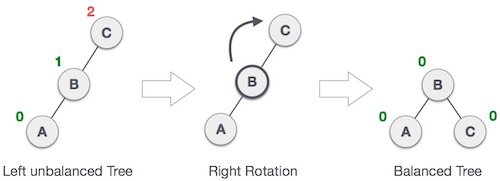
\includegraphics[scale=.60]{images/avl_right_rotation.jpg}
\end{center}

As depicted, the unbalanced node becomes the right child of its left child by performing a right rotation.

\hypertarget{left-right-rotation}{%
\mysubsubsection{Left-Right Rotation}\label{left-right-rotation}}

Double rotations are slightly complex version of already explained versions of rotations. To understand them better, we should take note of each action performed while rotation. Let's first check how to perform Left-Right rotation. A left-right rotation is a combination of left rotation followed by right rotation.

\begin{longtable}{| M{.20\textwidth} | p{.80\textwidth} |} 
% \begin{table}[H]
\hline
\textbf{State} & \textbf{Action} \\
\hline
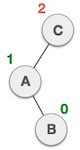
\includegraphics[scale=.40]{images/right_subtree_of_left_subtree.jpg} & A node has been inserted into the right subtree of the left subtree. This makes \textbf{C} an unbalanced node. These scenarios cause AVL tree to perform left-right rotation. \\ 
\hline
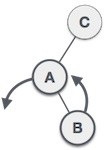
\includegraphics[scale=.40]{images/subtree_left_rotation.jpg} & We first perform the left rotation on the left subtree of \textbf{C}. This makes \textbf{A}, the left subtree of \textbf{B}. \\ 
\hline
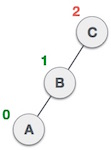
\includegraphics[scale=.40]{images/left_unbalanced_tree.jpg} & Node \textbf{C} is still unbalanced, however now, it is because of the left-subtree of the left-subtree. \\ 
\hline
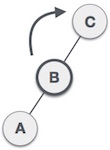
\includegraphics[scale=.40]{images/right_rotation.jpg} & We shall now right-rotate the tree, making \textbf{B} the new root node of this subtree. \textbf{C} now becomes the right subtree of its own left subtree. \\ 
\hline
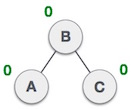
\includegraphics[scale=.40]{images/balanced_avl_tree.jpg} & The tree is now balanced. \\ 
\hline
\end{longtable}

\hypertarget{right-left-rotation}{%
\mysubsubsection{Right-Left Rotation}\label{right-left-rotation}}

The second type of double rotation is Right-Left Rotation. It is a
combination of right rotation followed by left rotation.

\begin{longtable}{| M{.20\textwidth} | p{.80\textwidth} |} 
% \begin{table}[H]
\hline
\textbf{State} & \textbf{Action} \\
\hline
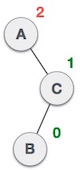
\includegraphics[scale=.40]{images/left_subtree_of_right_subtree.jpg} & A node has been inserted into the left subtree of the right subtree. This makes \textbf{A}, an unbalanced node with balance factor 2.\\
\hline
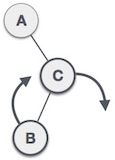
\includegraphics[scale=.40]{images/subtree_right_rotation.jpg} & First, we perform the right rotation along \textbf{C} node, making \textbf{C} the right subtree of its own left subtree \textbf{B}. Now, \textbf{B} becomes the right subtree of \textbf{A}. \\
\hline
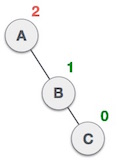
\includegraphics[scale=.40]{images/right_unbalanced_tree.jpg} & Node \textbf{A} is still unbalanced because of the right subtree of its right subtree and requires a left rotation.\\
\hline
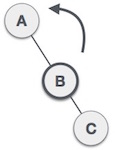
\includegraphics[scale=.40]{images/left_rotation.jpg} & A left rotation is performed by making \textbf{B} the new root node of the subtree. \textbf{A} becomes the left subtree of its right subtree \textbf{B}. \\
\hline
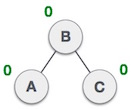
\includegraphics[scale=.50]{images/balanced_avl_tree.jpg} & The tree is now balanced.
\hline
\end{longtable}